%%%%%%%%%%%%%%%%%%%%%%%%%%%%%%%%%%%%%%%%%%%%%%%%%%%%%%%%%%%%%%%%%%%%%
%                                                                   %
%	CHAPTER TWO, FLECSPH.                                           %
%                                                                   %
%%%%%%%%%%%%%%%%%%%%%%%%%%%%%%%%%%%%%%%%%%%%%%%%%%%%%%%%%%%%%%%%%%%%%
\chapter{FleCSPH}

\section{Introduction}

\section{LANL and FleCSI}
FleCSI%HL : I guess we do not need extra footnote for flecsi so I comment out\footnote{\url{http://github.com/laristra/flecsi}}
~\cite{bergen2016flexible} is a compile-time configurable framework designed to support multi-physics application development. 
It is developed at the Los Alamos National Laboratory as part of the Los Alamos Ristra project. 
As such, FleCSI provides a very general set of infrastructure design patterns that can be specialized and extended to suit the needs of a broad variety of solver and data requirements. 
FleCSI currently supports multi-dimensional mesh topology, geometry, and adjacency information, as well as n-dimensional hashed-tree data structures, graph partitioning interfaces, and dependency closures.

FleCSI introduces a functional programming model with control, execution, and data abstractions that are consistent both with MPI and with state-of-the-art, task-based runtimes such as Legion\cite{bauer2012legion} and Charm++\cite{kale1993charm++}. 
The abstraction layer insulates developers from the underlying runtime, while allowing support for multiple runtime systems including conventional models like asynchronous MPI.

The intent is to provide developers with a concrete set of user-friendly programming tools that can be used now, while allowing flexibility in choosing runtime implementations and optimization that can be applied to future architectures and runtimes.

FleCSI's control and execution models provide formal nomenclature for describing poorly understood concepts such as kernels and tasks. 
FleCSI's data model provides a low-buy-in approach that makes it an attractive option for many application projects, as developers are not locked into particular layouts or data structure representations.

FleCSI currently provides a parallel but not distributed implementation of Binary, Quad and Oct-tree topology. 
This implementation is base on space filling curves domain decomposition, the Morton order. 
The current version allows the user to specify the code main loop and the data distribution requested. 
The data distribution feature is not available for the tree data structure needed in our SPH code and we provide it in the FleCSPH implementation. 
The next step will be to incorporate it directly from FleCSPH to FleCSI as we reach a decent level of performance.
As FleCSI is an on-development code the structure may change in the future and we keep track of these updates in FleCSPH.


Based on FleCSI the intent is to provide a binary, quad and oct-tree data structure and the methods to create, search and share information for it. 
In FleCSPH this will be dedicated, apply and tested on the SPH method. 
In this part we first present the domain decomposition, based on space filling curves, and the tree data structure.
We describe the HDF5 files structure used for the I/O.
Then we describe the distributed algorithm for the data structure over the MPI processes. 

\section{FleCSPH implementation}

\subsection{Domain decomposition}
\label{sec:domain_decomposition}
The number of particles can be high and represent a huge amount of data that does not fit in a single node memory. 
This implies the distribution of the particles over several computational nodes. 
As the particles moves during the simulation the static distribution is not possible and they have to be redistributed at some point in the execution. 
Furthermore, this distribution need to keep local particles in the same computation node to optimize the exchanges and computation itself.

A common approach is to distribute the particles over computational nodes using \textit{space filling curves} like in \cite{warren20132hot,springel2005cosmological,bedorf201424}. 
It intends to assign to each particle a key which is based on its spacial coordinates, then sorting particles based on those keys keeps particles grouped locally.
Many space filling curves exists: Morton, Hilbert, Peano, Moore, Gosper, etc.\

This domain decomposition is used in several layers for our implementation. 
On one hand, to spread the particles over all the MPI processes and provide a decent load balancing regarding the number of particles. 
On the other hand, it is also used locally to store efficiently the particles and provide a $O(N log(N))$ neighbor search complexity, instead of $O(N^2)$, using a tree representation describe in part \ref{sec:trees}. 

Several space filling curves can fit our purposes:
\subsubsection*{The Morton curves} \cite{morton1966computer}, or Z-Order, is the most spread method. 
This method can produce irregular shape domain decomposition like shown in green on Fig.~\ref{fig:space_filling}. 
The main advantage is to be fast to compute, the key is made by interlacing directly the X, Y and Z bits without rotations. 
\subsubsection*{The Hilbert curves} \cite{sagan2012space} are constructed by interlacing bits but also adding rotation based on the Gray code.
This work is based on the Peano curves and also called Hilber-Peano. 
The construction is more complicated than Morton but allows a better distribution. 

\begin{figure}
\centering
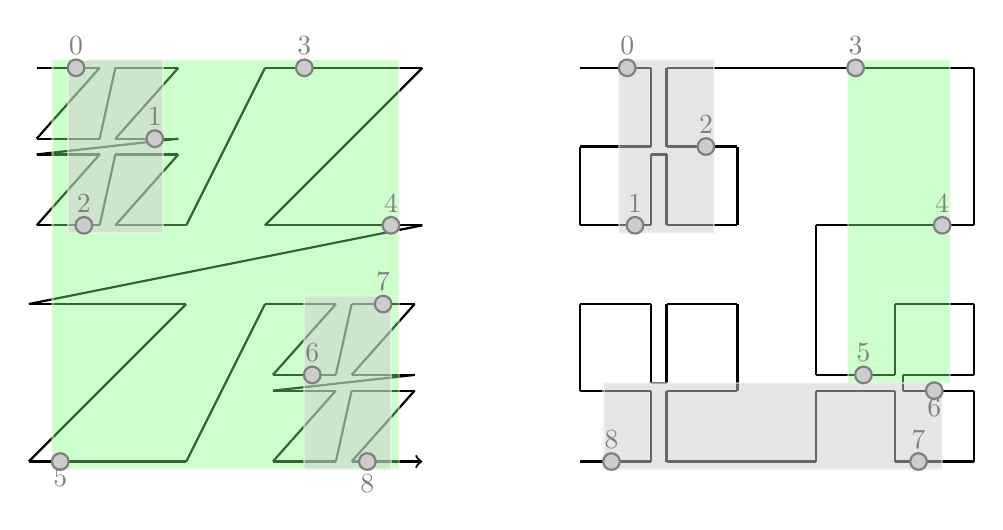
\begin{tikzpicture}[thick]
%\draw[black!50,fill=black!30] (2,2) circle (5pt);
% Morton
\draw[-] (.1,5) -- (.9,5);
\draw[-] (.9,5) -- (.1,4.1);
\draw[-] (.1,4.1) -- (.9,4.1);
\draw[-] (.9,4.1) -- (1.1,5);
\draw[-] (1.1,5) -- (1.9,5);
\draw[-] (1.9,5) -- (1.1,4.1);
\draw[-] (1.1,4.1) -- (1.9,4.1);
\draw[-] (1.9,4.1) -- (0.1,3.9);
\draw[-] (.1,3.9) -- (.9,3.9);
\draw[-] (.9,3.9) -- (.1,3);
\draw[-] (.1,3) -- (.9,3);
\draw[-] (.9,3) -- (1.1,3.9);
\draw[-] (1.1,3.9) -- (1.9,3.9);
\draw[-] (1.9,3.9) -- (1.1,3);
\draw[-] (1.1,3) -- (2,3);

\draw[-] (2,3) -- (3,5);
\draw[-] (3,5) -- (5,5);
\draw[-] (5,5) -- (3,3);
\draw[-] (3,3) -- (5,3);
\draw[-] (5,3) -- (0,2);
\draw[-] (0,2) -- (2,2);
\draw[-] (2,2) -- (0,0);
\draw[-] (0,0) -- (2,0);
\draw[-] (2,0) -- (3,2);

\draw[-] (3,2) -- (3.9,2);
\draw[-] (3.9,2) -- (3.1,1.1);
\draw[-] (3.1,1.1) -- (3.9,1.1);
\draw[-] (3.9,1.1) -- (4.1,2);
\draw[-] (4.1,2) -- (4.9,2);
\draw[-] (4.9,2) -- (4.1,1.1);
\draw[-] (4.1,1.1) -- (4.9,1.1);
\draw[-] (4.9,1.1) -- (3.1,.9);
\draw[-] (3.1,.9) -- (3.9,.9);
\draw[-] (3.9,.9) -- (3.1,0);
\draw[-] (3.1,0) -- (3.9,0);
\draw[-] (3.9,0) -- (4.1,0.9);
\draw[-] (4.1,0.9) -- (4.9,0.9);
\draw[-] (4.9,0.9) -- (4.1,0);
\draw[->] (4.1,0) -- (5,0);

% Hilbert
\draw[-] (7,5) -- (7.9,5);
\draw[-] (7.9,5) -- (7.9,4);
\draw[-] (7.9,4) -- (7,4);
\draw[-] (7,4) -- (7,3);
\draw[-] (7,3) -- (7.9,3);
\draw[-] (7.9,3) -- (7.9,3.9);
\draw[-] (7.9,3.9) -- (8.1,3.9);
\draw[-] (8.1,3.9) -- (8.1,3);
\draw[-] (8.1,3) -- (9,3);
\draw[-] (9,3) -- (9,4);
\draw[-] (9,4) -- (8.1,4);
\draw[-] (8.1,4) -- (8.1,5);
\draw[-] (8.1,5) -- (9,5);

\draw[-] (9,5) -- (10,5);
\draw[-] (10,5) -- (12,5);
\draw[-] (12,5) -- (12,3);
\draw[-] (12,3) -- (10,3);
\draw[-] (10,3) -- (10,2);

\draw[-] (10,2) -- (10,1.1);
\draw[-] (10,1.1) -- (11,1.1);
\draw[-] (11,1.1) -- (11,2);
\draw[-] (11,2) -- (12,2);
\draw[-] (12,2) -- (12,1.1);
\draw[-] (12,1.1) -- (11.1,1.1);
\draw[-] (11.1,1.1) -- (11.1,.9);
\draw[-] (11.1,.9) -- (12,.9);
\draw[-] (12,.9) -- (12,0);
\draw[-] (12,0) -- (11,0);
\draw[-] (11,0) -- (11,.9);
\draw[-] (11,.9) -- (10,.9);
\draw[-] (10,.9) -- (10,0);
\draw[-] (10,0) -- (9,0);

\draw[-] (9,0) -- (8.1,0);
\draw[-] (8.1,0) -- (8.1,.9);
\draw[-] (8.1,.9) -- (9,.9);
\draw[-] (9,.9) -- (9,2);
\draw[-] (9,2) -- (8.1,2);
\draw[-] (8.1,2) -- (8.1,1);
\draw[-] (8.1,1) -- (7.9,1);
\draw[-] (7.9,1) -- (7.9,2);
\draw[-] (7.9,2) -- (7,2);
\draw[-] (7,2) -- (7,.9);
\draw[-] (7,.9) -- (7.9,.9);
\draw[-] (7.9,.9) -- (7.9,0);
\draw[-] (7.9,0) -- (7,0);

% Add the particles over it 
\draw[black!5,opacity=.4,fill=green!50] (.3,-.1) rectangle (4.7,5.1);
\draw[black!5,opacity=0.5,fill=black!20] (.5,2.9) rectangle (1.7,5.1);
\draw[black!5,opacity=0.5,fill=black!20] (3.5,-0.1) rectangle (4.6,2.1);
% P1
\draw[black!50,fill=black!20] (0.6,5) circle (3pt) node[yshift=1pt,above] {0};
\draw[black!50,fill=black!20] (1.6,4.1) circle (3pt) node[yshift=1pt,above] {1};
\draw[black!50,fill=black!20] (.7,3) circle (3pt) node[yshift=1pt,above] {2};
% rect 1 
\draw[black!50,fill=black!20] (3.5,5) circle (3pt) node[yshift=1pt,above] {3};
\draw[black!50,fill=black!20] (4.6,3) circle (3pt) node[yshift=1pt,above] {4};
\draw[black!50,fill=black!20] (.4,0) circle (3pt) node[yshift=1pt,below] {5};
% rect 1 
\draw[black!50,fill=black!20] (3.6,1.1) circle (3pt) node[yshift=1pt,above] {6};
\draw[black!50,fill=black!20] (4.5,2) circle (3pt) node[yshift=1pt,above] {7};
\draw[black!50,fill=black!20] (4.3,0) circle (3pt) node[yshift=-1pt,below] {8};
% rect 1 


% hilbert rectangles 
\draw[black!5,opacity=.4,fill=green!50] (10.4,1) rectangle (11.7,5.1);
\draw[black!5,opacity=0.5,fill=black!20] (7.5,2.9) rectangle (8.7,5.1);
\draw[black!5,opacity=0.5,fill=black!20] (7.3,-.1) rectangle (11.6,1);

% Hilbert particles
\draw[black!50,fill=black!20] (7.6,5) circle (3pt) node[yshift=1pt,above] {0};
\draw[black!50,fill=black!20] (7.7,3) circle (3pt) node[yshift=1pt,above] {1};
\draw[black!50,fill=black!20] (8.6,4) circle (3pt) node[yshift=1pt,above] {2};

\draw[black!50,fill=black!20] (10.5,5) circle (3pt) node[yshift=1pt,above] {3};
\draw[black!50,fill=black!20] (11.6,3) circle (3pt) node[yshift=1pt,above] {4};
\draw[black!50,fill=black!20] (10.6,1.1) circle (3pt) node[yshift=1pt,above] {5};

\draw[black!50,fill=black!20] (11.5,.9) circle (3pt) node[yshift=1pt,below] {6};
\draw[black!50,fill=black!20] (11.3,0) circle (3pt) node[yshift=1pt,above] {7};
\draw[black!50,fill=black!20] (7.4,0) circle (3pt) node[yshift=1pt,above] {8};



\end{tikzpicture}
%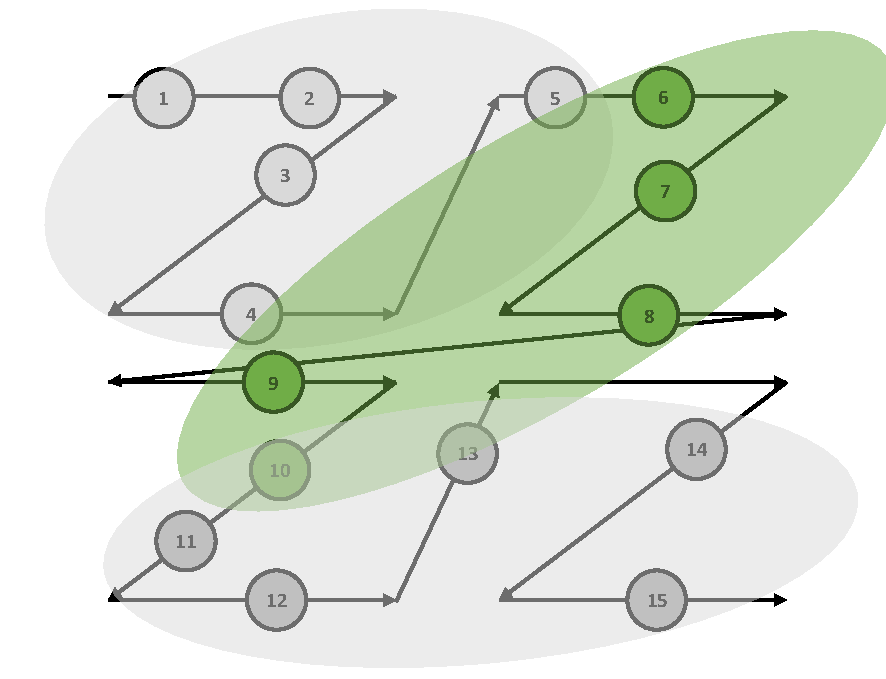
\includegraphics[scale=.28]{\locpath/figures/flecsph/morton_curve.pdf}
%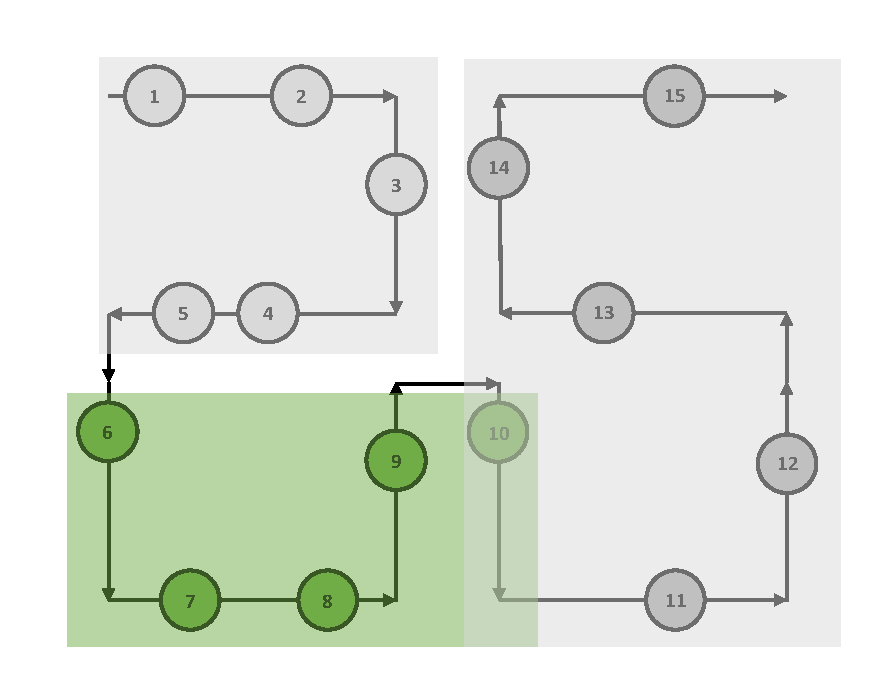
\includegraphics[scale=.28]{\locpath/figures/flecsph/hilbert_curve.pdf}
\caption{Morton and Hilbert space filling curves}
\label{fig:space_filling}
\end{figure}

On Fig.~\ref{fig:space_filling}, the Morton (left) and Hilbert (right) space-filling curves are represented in this example.
The particles are distributed over 3 processes. 
The set of particles of the second process appears in green. 
As we can see there are discontinuities on the Morton case due to the Z-order "jump" over the space. 
This can lead to non-local particles and over-sharing of particles that will not be needed during the computation.
In the Hilbert curve, the locality over the processes is conserved.

In this first implementation of FleCSPH we used the Morton ordering due to the computational cost. 
The next step of this work is to compare the computation time of different space filing curves. 

Technically the keys are generated for each particle at each iteration because their position is expected to change over time. 
To be more efficient, the keys can stay the same during several steps and the final comparison can be made on the real particles positions. 
This increase the search time but allows less tree reconstructions.

We use 64 bits to represent the keys to avoid conflicts.
The FleCSI code allows us to use a combination of memory words to reach the desired size of keys (possibly more than 64 bits) but this will cost in memory occupancy. 
The particle keys are generated by normalizing the space and then converting the floating-point representation to a 64 bits integer for each dimensions. 
Then the Morton interlacing is done and the keys are created. 
Unfortunately in some arrangements, like isolated particles, or scenarios with very close particles, the keys can be either badly distributed or duplicate keys can appear. 
Indeed, if the distance between two particles is less than $2^{-64} \approx 1$e+$20$, in a normalized space, the key generated through the algorithm will be the same. 
This problem is then handle during the particle sort and then the tree generation. 
In both case two particles can be differentiate based on their unique ID generated at the beginning execution. 

\subsection{Hierarchical trees}
\label{sec:trees}

The method we use for the tree data structure creation and research comes from Barnes-Hut trees presented in \cite{barnes1986hierarchical,barnes1990modified}. 
By reducing the search complexity from $O(N^2)$ for direct summation to $O(Nlog(N))$ it allows us to do very large simulations with billions of particles. 
It also allows the use of the tree data structure to compute gravitation using multipole methods.

We consider binary trees, for 1 dimension, quad-trees, for 2 dimensions, and oct-trees, for 3 dimensions. 
The construction of those trees is directly based on the domain decomposition using keys and space-filling curve presented in section \ref{sec:domain_decomposition}. 

\begin{figure}
\centering
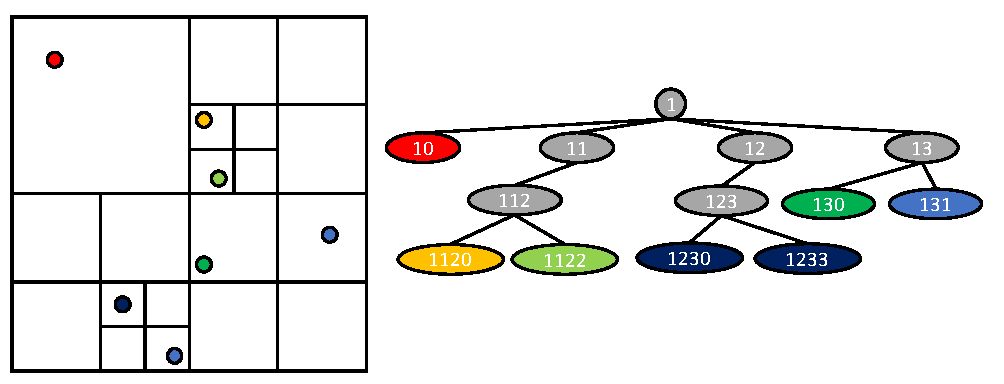
\includegraphics[width=\columnwidth]{\locpath/figures/flecsph/quadtree}
\caption{Quadtree, space and data representation}
\label{fig:quadtree}
\end{figure}

As explain in the previous section, we use 64 bits keys.
That give us up to $63$, $31$ and $21$ levels in the tree for respectively 1, 2 and 3 dimensions. 
As presented on Fig.~\ref{fig:quadtree} the first bit is use to represent the root of the tree, $1$.
This allows us to have up to $2^{63}$ different keys and unique particles.  

\subsubsection{Tree generation}

After each particle get distributed on its final process using its space-filling curve key, we can recursively construct the tree.
Each particle is added and the branches are created recursively if there is an intersection between keys. 
Starting from the root of key "1" the branches are added at each levels until the particles are reached.
An example of a final tree is shown on Fig.~\ref{fig:quadtree}.

\subsubsection{Tree search}

When all the particles have been added, the data regarding the tree nodes are computed with a bottom up approach. 
Summing up the mass, position called Center of Mass (COM), and the boundary box of all sub-particles of this tree node.

For the search algorithm the basic idea would be to do a tree traversal for all the particles and once we reach a particle or a node that interact with the particle smoothing length, add it for computation or in a neighbor list. 
Beside of being easy to implement and to use in parallel this algorithm requires a full tree traversal for every particle and will not take advantage of the particles' locality.

Our search algorithm, presented on Algorithm~\ref{alg:find_nodes}, is a two step algorithm like in Barnes trees: First create the interaction lists and then using them on the sub-tree particles. 
In the first step we look down for nodes with a target sub-mass of particles $tmass$. 
Then for those branches we compute an interaction list and continue the recursive tree search. 
When a particle is reached, we compute the physics using the interaction list as the neighbors. 
The interaction list is computing using an opening-angle criterion comparing the boundary box and an user define angle. 
In this way we will not need a full tree traversal for each particle but a full tree traversal for every group of particles.

\begin{algorithm}
\caption{Tree search algorithm}\label{alg:find_nodes}
\begin{algorithmic}[1]
\Procedure{find\_nodes}{}
\State stack $stk \leftarrow$ root
\While{not\_empty($stk$)} 
	\State branch $b \leftarrow$ $stk$.pop() 
	\If{$b$ is leaf} 
		\For{\textbf{each} particles $p$ of $b$}
			\State $apply\_sub\_tree$($p$,$interaction\_list$($p$))
		\EndFor
	\Else
		\For{\textbf{each} child branch $c$ of $b$}
			\State $stk$.push($c$)
		\EndFor
	\EndIf
\EndWhile
\EndProcedure
\State
\Procedure{apply\_sub\_tree}{node $n$, node-list $nl$}
\State stack $stk \leftarrow$ $n$
\While{not\_empty($stk$)} 
	\State branch $b \leftarrow$ $stk$.pop() 
	\If{$b$ is leaf} 
		\For{\textbf{each} particles $p$ of $b$}
			\State $apply\_physics$($p$,$nl$)
		\EndFor
	\Else
		\For{\textbf{each} child branch $c$ of $b$}
			\State $stk$.push($c$)
		\EndFor
	\EndIf
\EndWhile
\EndProcedure
\State
\Function{interaction\_list}{node $n$}
\State stack $stk \leftarrow$ root
\State node-list $nl$ $\leftarrow$ $\emptyset$
\While{not\_empty($stk$)} 
	\State branch $b \leftarrow$ $stk$.pop() 
	\If{$b$ is leaf} 
		\For{\textbf{each} particles $p$ of $b$}
			\If{within()}
				\State $nl$ $\leftarrow$ $nl$ + $p$
			\EndIf
		\EndFor
	\Else
		\For{\textbf{each} child branch $c$ of $b$}
			\If{$mac$($c$,$angle$)}
				\State $nl$ $\leftarrow$ $nl$ + $c$
			\Else				
				\State $stk$.push($c$)
			\EndIf	
		\EndFor
	\EndIf
\EndWhile
\EndFunction
\end{algorithmic}
\end{algorithm}

\subsection{Distribution strategies}

The previous section presented the tree data structure that can be use locally on every node. 
The distribution layer is added on top of it, keeping each sub-tree on the computation nodes. 
The current version of FleCSPH is still based on synchronous communications using the Message Passing Interface (MPI). 

\begin{algorithm}
\caption{Main algorithm}\label{alg:main_distributed}
\begin{algorithmic}[1]
\Procedure{specialization\_driver}{input data file $f$}
\State Read $f$ in parallel 
\State Set physics constant from $f$
\While{iterations}
\State Distribute the particles using distributed quick sort\label{alg_main:qsort}
\State Compute total range 
\State Generate the local tree
\State Share branches\label{alg_main:share_branches}
\State Compute the ghosts particles\label{alg_main:cp_ghosts}
\State Update ghosts data\label{alg_main:up_ghosts}
\State \textit{PHYSICS}
\State Update ghosts data
\State \textit{PHYSICS}
\State Distributed output to file 
\EndWhile
\EndProcedure
\end{algorithmic}
\end{algorithm}


The main distributed algorithm is presented on algorithm \ref{alg:main_distributed}:

\subsubsection{Particle distribution}

\begin{figure*}
\centering
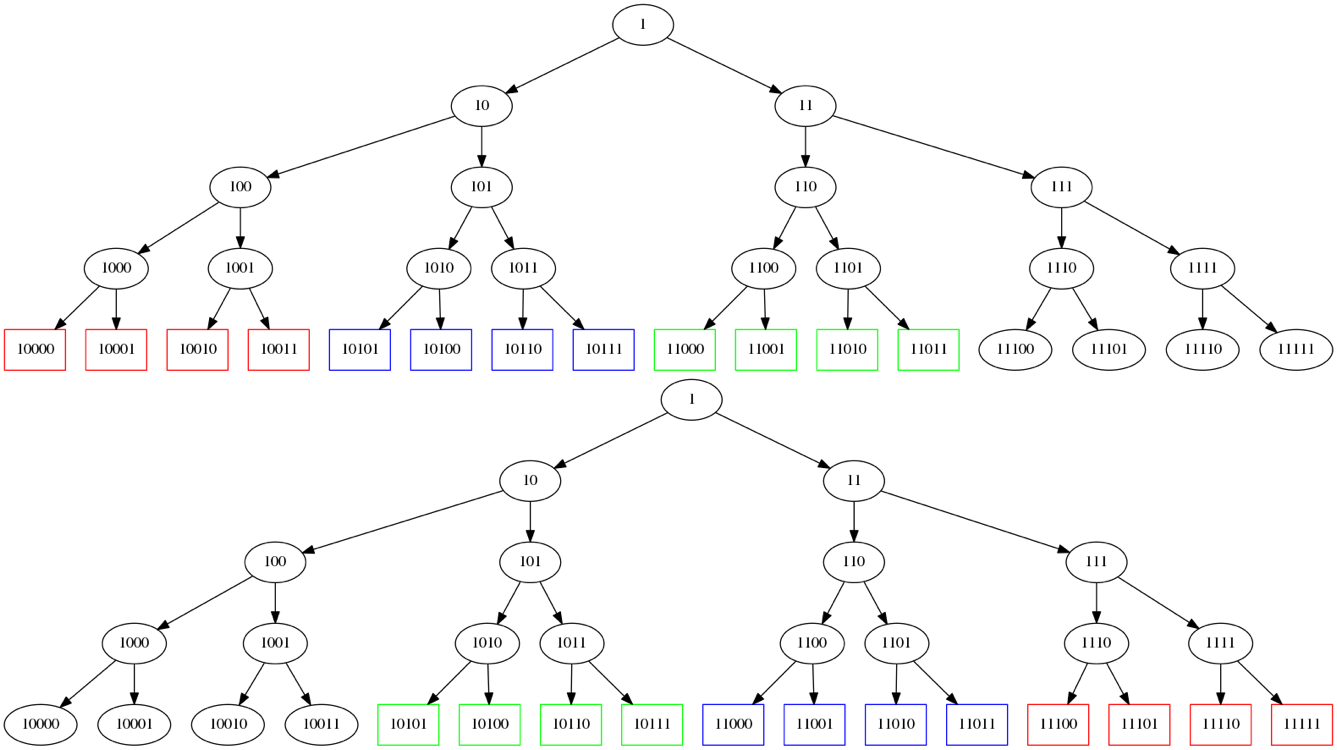
\includegraphics[width=\textwidth]{\locpath/figures/flecsph/algo.png}
\caption{Binaries tree for a 2 processes system. Exclusive, Shared and Ghosts particles resp. red, blue, green.}
\label{fig:big_tree}
\end{figure*}

The sort step, line \ref{alg_main:qsort}, is base on a distributed quick sort algorithm. 
The keys are generated using the Morton order described in part \ref{sec:domain_decomposition}. 
As we associate a unique number to each particle we are able to sort them using the keys and, in case of collision keys, using their unique ID. 
This gives us a global order for the particles. 
Each process sends to a master node (or submaster for larger cases) a sample of its keys. 
We determined this size to be 256 KB of key data per process for our test cases but it can be refined for larger simulations. 
Then the master determines the general ordering for all the processes and shares the pivots. 
Then each process locally sort its local keys and, in a global communication step, the particles are distributed to the process on which they belong. 
This algorithm gives us a good partition in term of number of particles. 
But some downside can be identified:
\begin{itemize}
	\item The ordering may not be balanced in term of number of particles per processes. But by optimizing the number of data exchanged to the master can lead to better affectation. 
	\item The load balance also depend on the number of neighbors of each particle. If a particle get affected a poor area with large space between the particles, this can lead to bad load balancing too. 
\end{itemize}
This is why we also provide another load balancing based on the particles neighbors. 
Depending on the user problem, the choice can be to distribute the particles on each processes regarding the number of neighbors, having the same amount of physical computation to perform on each processes. 

After this first step, the branches are shared between the different processes, line \ref{alg_main:share_branches}. 
Every of them send to its neighbors several boundaries boxes, defined by the user. 
Then particles from the neighbors are computed, exchanged and added in the local tree. 
Those particles are labeled as NON\_LOCAL particles. 
At this point a particle can be referenced as: EXCLUSIVE: will never be exchanged and will only be used on this process; SHARED: may be needed by another process during the computation; GHOSTS: particles information that the process need to retrieve from another process. 
An example is given for 2 processes on Fig.~\ref{fig:big_tree}.

\subsubsection{Exchange Shared and Ghosts particles}

The previous distribution shares the particles and the general information about neighbors particles. 
Then each process is able to do synchronously or asynchronously communications to gather distant particles. 
In the current version of FleCSPH an extra step is required to synchronously share data of the particles needed during the next tree traversal and physics part. 
Then after this step, the ghosts data can be exchanged as wanted several times during the same time step. 

\subsection{I/O}
Regarding the high number of particles, an efficient, parallel and distributed I/O implementation is required. 
Several choices were available but we wanted a solution that can be specific for our usage. 
The first requirement is to allow the user to work directly with the Paraview visualization tool and splash\footnote{\url{http://users.monash.edu.au/~dprice/splash/}}~\cite{price2007splash}.

We base this first implementation on HDF5~\cite{folk1999hdf5} file structure with H5Part and H5Hut~\cite{howison2010h5hut}. 
HDF5 support MPI runtime with distributed read and write in a single or multiple files. 
We added the library H5hut to add normalization in the code to represent global data, steps, steps data and the particles data for each steps.
The I/O code was developed internally at LANL and provides a simple way to write and read the data in H5Part format. 
The usage of H5Hut to generate H5part data files allows us to directly read the output in Paraview without using a XDMF descriptor like requested in HDF5 format.


\section{Conclusion}